% 
% Author: Izaak Niksan - 1002659777
%
%%%%%%%%%%%%%%%%%%%%%%%%%%%%%%%%%%%%%%%%
% Programming/Coding Assignment
% LaTeX Template
%
% This template has been downloaded from:
% http://www.latextemplates.com
%
% Original author:
% Ted Pavlic (http://www.tedpavlic.com)
%
% Note:
% The \lipsum[#] commands throughout this template generate dummy text
% to fill the template out. These commands should all be removed when 
% writing assignment content.
%
% This template uses a Perl script as an example snippet of code, most other
% languages are also usable. Configure them in the "CODE INCLUSION 
% CONFIGURATION" section.
%
%%%%%%%%%%%%%%%%%%%%%%%%%%%%%%%%%%%%%%%%%
% 
%----------------------------------------------------------------------------------------
%   PACKAGES AND OTHER DOCUMENT CONFIGURATIONS
%----------------------------------------------------------------------------------------

\documentclass{article}

\usepackage{fancyhdr} % Required for custom headers
\usepackage{lastpage} % Required to determine the last page for the footer
\usepackage{extramarks} % Required for headers and footers
\usepackage[usenames,dvipsnames]{color} % Required for custom colors
\usepackage{graphicx} % Required to insert images
\usepackage{subcaption}
\usepackage{listings} % Required for insertion of code
\usepackage{courier} % Required for the courier font
\usepackage{lipsum} % Used for inserting dummy 'Lorem ipsum' text into the template
\graphicspath{ {latex_images/} }

% Margins
\topmargin=-0.45in
\evensidemargin=0in
\oddsidemargin=0in
\textwidth=6.5in
\textheight=9.0in
\headsep=0.25in

\linespread{1.1} % Line spacing

% Set up the header and footer
\pagestyle{fancy}
\lhead{\hmwkAuthorName} % Top left header
\chead{\hmwkClass\ (\hmwkClassTime): \hmwkTitle} % Top center head
%\rhead{\firstxmark} % Top right header
\lfoot{\lastxmark} % Bottom left footer
\cfoot{} % Bottom center footer
\rfoot{Page\ \thepage\ of\ \protect\pageref{LastPage}} % Bottom right footer
\renewcommand\headrulewidth{0.4pt} % Size of the header rule
\renewcommand\footrulewidth{0.4pt} % Size of the footer rule

\setlength\parindent{0pt} % Removes all indentation from paragraphs

%----------------------------------------------------------------------------------------
%   CODE INCLUSION CONFIGURATION
%----------------------------------------------------------------------------------------

\definecolor{MyDarkGreen}{rgb}{0.0,0.4,0.0} % This is the color used for comments
\lstloadlanguages{Perl} % Load Perl syntax for listings, for a list of other languages supported see: ftp://ftp.tex.ac.uk/tex-archive/macros/latex/contrib/listings/listings.pdf
\lstset{language=Perl, % Use Perl in this example
        frame=single, % Single frame around code
        basicstyle=\small\ttfamily, % Use small true type font
        keywordstyle=[1]\color{Blue}\bf, % Perl functions bold and blue
        keywordstyle=[2]\color{Purple}, % Perl function arguments purple
        keywordstyle=[3]\color{Blue}\underbar, % Custom functions underlined and blue
        identifierstyle=, % Nothing special about identifiers                                         
        commentstyle=\usefont{T1}{pcr}{m}{sl}\color{MyDarkGreen}\small, % Comments small dark green courier font
        stringstyle=\color{Purple}, % Strings are purple
        showstringspaces=false, % Don't put marks in string spaces
        tabsize=5, % 5 spaces per tab
        %
        % Put standard Perl functions not included in the default language here
        morekeywords={rand},
        %
        % Put Perl function parameters here
        morekeywords=[2]{on, off, interp},
        %
        % Put user defined functions here
        morekeywords=[3]{test},
        %
        morecomment=[l][\color{Blue}]{...}, % Line continuation (...) like blue comment
        numbers=left, % Line numbers on left
        firstnumber=1, % Line numbers start with line 1
        numberstyle=\tiny\color{Blue}, % Line numbers are blue and small
        stepnumber=5 % Line numbers go in steps of 5
}

% Creates a new command to include a perl script, the first parameter is the filename of the script (without .pl), the second parameter is the caption
\newcommand{\perlscript}[2]{
\begin{itemize}
\item[]\lstinputlisting[caption=#2,label=#1]{#1.pl}
\end{itemize}
}

%----------------------------------------------------------------------------------------
%   DOCUMENT STRUCTURE COMMANDS
%   Skip this unless you know what you're doing
%----------------------------------------------------------------------------------------

% Header and footer for when a page split occurs within a problem environment
\newcommand{\enterProblemHeader}[1]{
%\nobreak\extramarks{#1}{#1 continued on next page\ldots}\nobreak
%\nobreak\extramarks{#1 (continued)}{#1 continued on next page\ldots}\nobreak
}

% Header and footer for when a page split occurs between problem environments
\newcommand{\exitProblemHeader}[1]{
%\nobreak\extramarks{#1 (continued)}{#1 continued on next page\ldots}\nobreak
%\nobreak\extramarks{#1}{}\nobreak
}

\setcounter{secnumdepth}{0} % Removes default section numbers
\newcounter{homeworkProblemCounter} % Creates a counter to keep track of the number of problems
\setcounter{homeworkProblemCounter}{-1}

\newcommand{\homeworkProblemName}{}
\newenvironment{homeworkProblem}[1][Problem \arabic{homeworkProblemCounter}]{ % Makes a new environment called homeworkProblem which takes 1 argument (custom name) but the default is "Problem #"
\stepcounter{homeworkProblemCounter} % Increase counter for number of problems
\renewcommand{\homeworkProblemName}{#1} % Assign \homeworkProblemName the name of the problem
\section{\homeworkProblemName} % Make a section in the document with the custom problem count
\enterProblemHeader{\homeworkProblemName} % Header and footer within the environment
}{
\exitProblemHeader{\homeworkProblemName} % Header and footer after the environment
}

\newcommand{\problemAnswer}[1]{ % Defines the problem answer command with the content as the only argument
\noindent\framebox[\columnwidth][c]{\begin{minipage}{0.98\columnwidth}#1\end{minipage}} % Makes the box around the problem answer and puts the content inside
}

\newcommand{\homeworkSectionName}{}
\newenvironment{homeworkSection}[1]{ % New environment for sections within homework problems, takes 1 argument - the name of the section
\renewcommand{\homeworkSectionName}{#1} % Assign \homeworkSectionName to the name of the section from the environment argument
\subsection{\homeworkSectionName} % Make a subsection with the custom name of the subsection
\enterProblemHeader{\homeworkProblemName\ [\homeworkSectionName]} % Header and footer within the environment
}{
\enterProblemHeader{\homeworkProblemName} % Header and footer after the environment
}

%----------------------------------------------------------------------------------------
%   NAME AND CLASS SECTION
%----------------------------------------------------------------------------------------

\newcommand{\hmwkTitle}{Project\ \#1} % Assignment title
\newcommand{\hmwkDueDate}{Monday,\ March\ 19,\ 2018} % Due date
\newcommand{\hmwkClass}{CSC411} % Course/class
\newcommand{\hmwkClassTime}{Thursday 6-9 pm} % Class/lecture time
\newcommand{\hmwkAuthorName}{Izaak Niksan} % Your name

%----------------------------------------------------------------------------------------
%   TITLE PAGE
%----------------------------------------------------------------------------------------

\title{
\vspace{2in}
\textmd{\textbf{\hmwkClass:\ \hmwkTitle}}\\
\normalsize\vspace{0.1in}\small{Due\ on\ \hmwkDueDate}\\
\vspace{0.1in}
\vspace{3in}
}

\author{\textbf{\hmwkAuthorName}}
\date{} % Insert date here if you want it to appear below your name

%----------------------------------------------------------------------------------------

\begin{document}

\maketitle
\clearpage
\textbf{Part 1)}\\
Upon first glance, one striking difference between the datasets is that the real articles appear to have significantly longer headlines on average. In terms of words that seem to appear more frequently in a specific dataset, the words \textit{hillary}, \textit{russia}, and \textit{victory} immediately stick out. The word \textit{hillary} appears 150 times in fake articles but only 24 times in real articles. The word \textit{russia} appears 45 times in fake articles and 77 times in real articles. The word \textit{victory} appears 48 times in fake articles and 25 times in real articles.\\\\
\textbf{Part 2)}\\
First, the data was separated into different sets by running the \textit{splitting\_datasets.py} script. This script parses the provided fake and real headlines and dumps various dictionaries into pickle files for easy access in future parts. The training set comprises 70\% of the headlines, the validation set 15\%, and the test set 15\%. These dictionaries contain words as keys, and the number of times each word appears as values.\\

In \textit{part2.py}, the Naive Bayes classifier was implemented. The code for the function is seen below. As noted in the project handout, it is undesirable to multiply many small floating point values together since approximations in their digital representations eventually lead to very inaccurate results. Instead, when implementing the classifier, a sum of logs was used instead. More specifically, when evaluating $$P(C|headline)=\frac{P(headline|C)P(C)}{P(headline)}=\frac{P(C)\Pi_{i}P(word_i|C)}{P(headline)},$$ instead of explicitly computing the term on the right, since the end goal was to determine which of $P(fake|headline)$ or $P(real|headline)$ was larger, it was sufficient to maximize the term on the right. Thus, since exponential functions are strictly increasing or decreasing and the term in the denominator is a constant, the term on the right was replaced with 
$log(P(headline))+\sum_{i}log(P(word_i|C))$.\\

One additional note is that, as described in the the lecture slides, "virtual examples" were added to the training set to avoid the case where the count of a word is 0. This was done by including two hyperparameters: $m$ and $p\_hat$. Using these, $P(word_i|C)$ was computed as follows:
$$P(word_i|C)=\frac{count(word_i,C) + m*p\_hat}{count(C)+m} $$ if $word_i$ appears in the headline, and otherwise as
$$P(word_i|C)=1-\frac{count(word_i,C) + m*p\_hat}{count(C)+m} $$
The ideal values for $m$ and $p\_hat$ were determined to be 1 and 0.35 respectively. They were optimized using the validation set; m was varied through integer values between 1 and 10, and p\_hat was varied through multiples of 0.05 between 0.05 and 1. The code for this optimization is also found in \textit{part2.py}.\\

The performance of the classifier on the training set and test set were 96.4\% and 84.9\% respectively.\\
\begin{lstlisting}[language=Python, caption=Naive Bayes Classifier]
def naive_bayes_istrue(headline,real,fake,real_count,fake_count,m,p_hat):
    '''
    Inputs:
        headline:    New headline which will be classified as real or fake. It 
                     is assumed that the headline is already cleanly processed.
        real:        Dictionary with keys as words which appear in real  
                     headlines and values as the number of times the words 
                     appear.
        fake:        Same type of dictionary but for fake headlines.
        real_count:  Number of real headlines.
        fake_count:  Number of fake headlines.
        m:           Number of virtual examples added to the sets.
        p_hat:       Prior probability. 
        
    Output:
        Boolean value, with true being true and false being fake
    '''
    
    line=headline
    line=line.rstrip('\n')
    temp=line.split(' ') # words contains all the words in the headline
    
    #remove any duplicated words in the headline:
    words=[]
    [words.append(item) for item in temp if item not in words]

    preal=real_count/(real_count+fake_count) #p(real)
    pfake=fake_count/(real_count+fake_count) #p(fake)
    real_prob=0 #Probability that headline is real
    fake_prob=0 #Probability that headline is fake
    
    #First calculate the probability that headline is real
    for key in real:
        if key in words:
            real_prob+=log((real[key] + m*p_hat)/(real_count+m))
        else:
            real_prob+=log(1-(real[key] + m*p_hat)/(real_count+m))
    real_prob+=log(preal)
    
    #Now calculate the probability that headline is fake
    for key in fake:
        if key in words:
            fake_prob+=log((fake[key]+m*p_hat)/(fake_count+m))
        else:
            fake_prob+=log(1-(fake[key]+m*p_hat)/(fake_count+m))
    
    fake_prob+=log(pfake)

    #At this point, we have been summing the log probabilities. We could 
    #exponentiate then divide by the normalization factor to get the actual
    #probabilites, but instead we just return the larger of the two values 
    #since we only care about relative sizes.
    
    if fake_prob>real_prob:
        return False
    else:
        return True
\end{lstlisting}
\newpage
\textbf{Part 3)}\\
\textit{a)} The presence of words which appear most frequently in real headlines contribute most towards predicting that the headline is real. Conversely, the absence of words which appear least frequently in real headlines contribute most towards predicting that he headline is real. The same logic applies to fake headlines.\\

The basis for this is the conditional probability formula, specifically the term in the numerator of Baye's Rule:
$$P(headline|C)=\Pi_{i}P(word_i|C)$$
For a given class, if the word appears in the headline then the factor in the multiplication corresponding to this word is calculated as the ratio of the number of times this word appears in headlines of this class to the number of total headlines of this class. Maximizing this ratio makes a larger contribution to increasing the overall probability. Similarly, if the word does not appear in the headline, the term instead becomes this same ratio, but subtracted from 1. Therefore, minimizing the ratio will lead to increasing the overall probability.\\

The 10 words whose presence most strongly predicts that the news is real are: \textit{trump, donald, to, us, in, trumps, on, of, says,} and \textit{for}.\\

The 10 words whose absence most strongly predicts that the news is real are: \textit{truths, pedo, ring, guerrilla, economist, avoid, scissors, ribbon, c,} and \textit{hypocrisy}.\\

The 10 words whose presence most strongly predicts that the news is fake are: \textit{trump, to, the, donald, for, in, of, and, a,} and \textit{on}.\\

The 10 words whose absence most strongly predicts that the news is fake are: \textit{avocado, grattan, date, jennett, backwards, jordan, vow, personnel, industrials,} and \textit{denuclearisation}.\\\\
\textit{b)} \textit{*It is assumed that this question is asking for the words whose presence most affects the probability*}\\
The 10 non-stopwords whose presence most strongly predicts that the news is real are: \textit{trump, donald, trumps, says, north, korea, election, clinton, ban,} and \textit{president}.\\
The 10 non-stopwords whose presence most strongly predicts that the news is fake are: \textit{trump, donald, hillary, clinton, election, just, president, new, america,} and \textit{obama}.\\

The explanation of why prevalence leads to increased probability is the same as what was described in part a).\\

\textit{c)} It usually makes sense to remove stopwords as they generally do not provide any meaningful information to the classifier since they are typically not relevant to the classification problem. In fact, having lots of stopwords in the datasets may actually confuse the classifier. However, in the rare case where one determines that the stopwords are actually relevant to the problem, then it may be useful to keep them in the datasets. One such example may be in the classification of spam emails; if it turns out to be the case that spam emails use many stopwords, since these emails generally do not have much meaningful content, then not removing them may be a wise decision.\newpage

\textbf{Part 4)}\\
In order to formulate this as a logistic regression classification problem, first the input vector $v\,\epsilon\, n\,x\,m$ (for $m$ headlines and $n$ inputs) was set up such that $v[k][z]=1$ when word $k$ appeared in headline $z$, else the value was 0.\\

As before, the headlines were cleaned up such that they became arrays of words, with spaces and newline characters removed. Some code from project 2 was reused. The inputs consisted off the words in the \textit{training set} only, since words which the classifier has never seen before cannot be used in any meaningful way. The output of the classifier is $y\,\epsilon\, 2\,x\,m$, such that $y[0][k]=1$ and $y[1][k]=0$ for a real headline, and the reverse for a fake one. In other words, it employs one-hot encoding. When an input is fed into the classifier, the index whose value is closest to 1 is taken as the classifier's guess.\\

For the gradient descent, alpha was 0.001, lambda was 0.8, and MAX\_ITERS was 10 000. As recommended on piazza, L2 regularization was used. It is noted that the value of lambda did not seem to significantly affect the performance. In order to tune lambda, the validation set was used. The lambda which led to the best classifier was chosen to be the optimal one. The optimizer started at lambda=0.1, ended at lambda=10, and increased by iterations of 0.1. Figure 1 displays the performance on the training and validation sets for lambda=10. Furthermore, the optimal alpha was higher than it was in the previous project.\\

Finally, as seen in Figure 2, the performance on the validation set seemed to peak at 75\%. This value seemed unexpectedly low, although regardless of the parameters of the algorithm the performance could never increase past this mark. It is also noted that the performance on the validation set seems to decline slightly even though the performance on the training set seems to continue to increase. This should be taken into consideration for the issue of overfitting; it may be preferred to end the descent after around 1000 iterations. Figure 3 displays the learning curves for MAX\_ITERS=1100.

\begin{center}
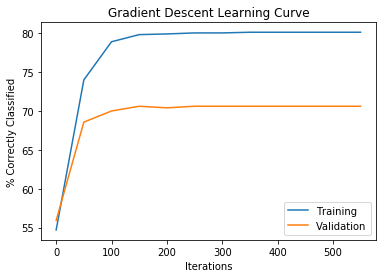
\includegraphics[width=13cm, height=8cm]{latex_images/part4_lambda10.png} 
\captionof{figure}{Learning Curves for a Logistic Regression Classifier on Training and Validation Sets. alpha=0.001, lambda=10, MAX\_ITERS=10 000}
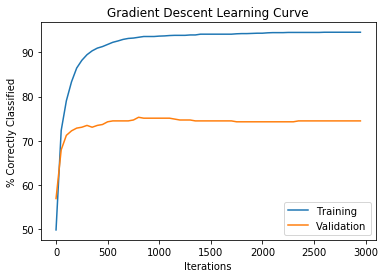
\includegraphics[width=13cm, height=8cm]{latex_images/part4_learningcurve_withval.png} 
\captionof{figure}{Learning Curves for a Logistic Regression Classifier on Training and Validation Sets. alpha=0.001, lambda=0.8, MAX\_ITERS=10 000}
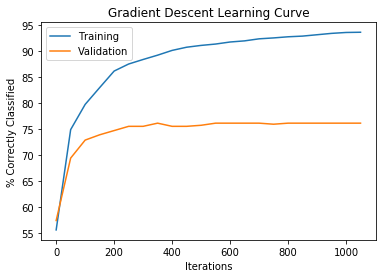
\includegraphics[width=13cm, height=8cm]{latex_images/part4_learningcurve_withval_1100.png} 
\captionof{figure}{Learning Curves for a Logistic Regression Classifier on Training and Validation Sets. alpha=0.001, lambda=0.8, MAX\_ITERS=1100}
\end{center}
\\
\textbf{Part 5)}\\
\textit{Logistic Regression:}\\
For logistic regression, the generalized multicase probability of the input being of class $i$ is 
$$p_i=\frac{exp(w_0^{(i)}+w_1^{(i)}x_1+...+w_k^{(i)}x_k)}{\sum_jexp(w_0^{(j)}+w_1^{(j)}x_1+...+w_k^{(j)}x_k)}>0.5$$
For the case of binary classification the expression can be written as
$$p_1=\frac{exp(o_1)}{exp(o_1)+exp(o_2)}=\frac{1}{1+exp(o_2-o_1)}>0.5,$$
where $o_i\equiv w_0^{(i)}+w_1^{(i)}x_1+...+w_k^{(i)}x_k$, and $p_1$ denotes the probability of the input being of class 1. Note that $p_1=1-p_2$. \\

Thus, rearranging, we require the following inequality to hold when deciding to classify as $y=1$:

$$1+exp(o_2-o_1)<2$$
$$exp(o_2-o_1)<1$$
Taking the natural log of both sides:
$$o_2-o_1=(w_0^{(2)}+w_1^{(2)}x_1+...+w_k^{(2)}x_k)-(w_0^{(1)}+w_1^{(1)}x_1+...+w_k^{(1)}x_k)<0$$
Grouping terms:
$$(w_0^{(2)}-w_0^{(1)})+(w_1^{(2)}-w_1^{(1)})x_1+...+(w_k^{(2)}-w_k^{(1)})x_k<0$$
Multiplying each side by -1:
$$(w_0^{(1)}-w_0^{(2)})+(w_1^{(1)}-w_1^{(2)})x_1+...+(w_k^{(1)}-w_k^{(2)})x_k=\theta_0+\theta_1I_1(x)+...+\theta_k I_k(x)>0$$
By observation, it is deduced that $\theta_j=(w_j^{(1)}-w_j^{(2)})$ and $I_j(x)=x_j$. This inequality must hold for classification as $y=1$, and must not hold for classification as $y=0$.\\

\textit{Naive Bayes:}\\
\\\\\\\\\\\\\\\\\\\\\\\\\\\\\\\\\









!!!!!!!!!!!!!!!!!!!!!!!!!!!!!!!!!!!! FINISH THIS PART !!!!!!!!!!!!!!!!!!!!!!!!!!!!!!!!!!\\\\\\\\\\\\\\\\\\\\\\\\\\\\\\\\\\\\\\\











\\\\
\textbf{Part 6)}\\

%----------------------------------------------------------------------------------------
\end{document}